\documentclass[10pt]{beamer}

\usetheme{metropolis}

\title{Introduction to Machine Learning}
\author{Bernd Bischl, Fabian Scheipl, Daniel Schalk\\}
\date{\url{https://github.com/compstat-lmu/lecture_i2ml}}
\begin{document}

% bilder größer aufziehen wenn moeglich / whitespace wegschneiden außen

\maketitle

\begin{frame}{Concept}

The course is organized as a digital lecture for ML beginners for statistics Bachelors and Data Science ESG student, which should be as self-contained and enable self-study as much as possible:

  \begin{itemize}
    \item
      Slides with lecture videos

    \item
      Interactive tutorials: Currently online quizzes and some very simple online 
      coding exercises

    \item
        Complemented by a week-long inverted-classroom block course 
            (code demos, slide discussion, supervised exercises)
    
        \item \textbf{Produce lecture like a piece of software / library: Literate programming, Github, collaborative, modular chunks, issues, pull requests, etc.}

  \end{itemize}
  

\end{frame}

\begin{frame}{Contents}

  \begin{itemize}
      \item Risk minimization
      \item Linear models, KNN, Naive Bayes
      \item Performance evaluation, cross-validation, ROC
      \item Decision trees, random forests
      \item Tuning
  \end{itemize}

\end{frame}

\begin{frame}{Prerequisites}
    The course is targeted at ML beginners with a basic, university level, education in maths
    \begin{itemize}
        \item Simple linear algebra
        \item Simple calculus
        \item Simple probability theory
        \item Some stats knowledge, you should now what mean, variance, bias, etc., is
            (Linear) Modelling from a stats perspective can help, but is not required, we sometimes compare to that
        \item Working knowledge of R
    \end{itemize}
\end{frame}

\begin{frame}{Concept - Lecture Videos}

  \begin{center}
      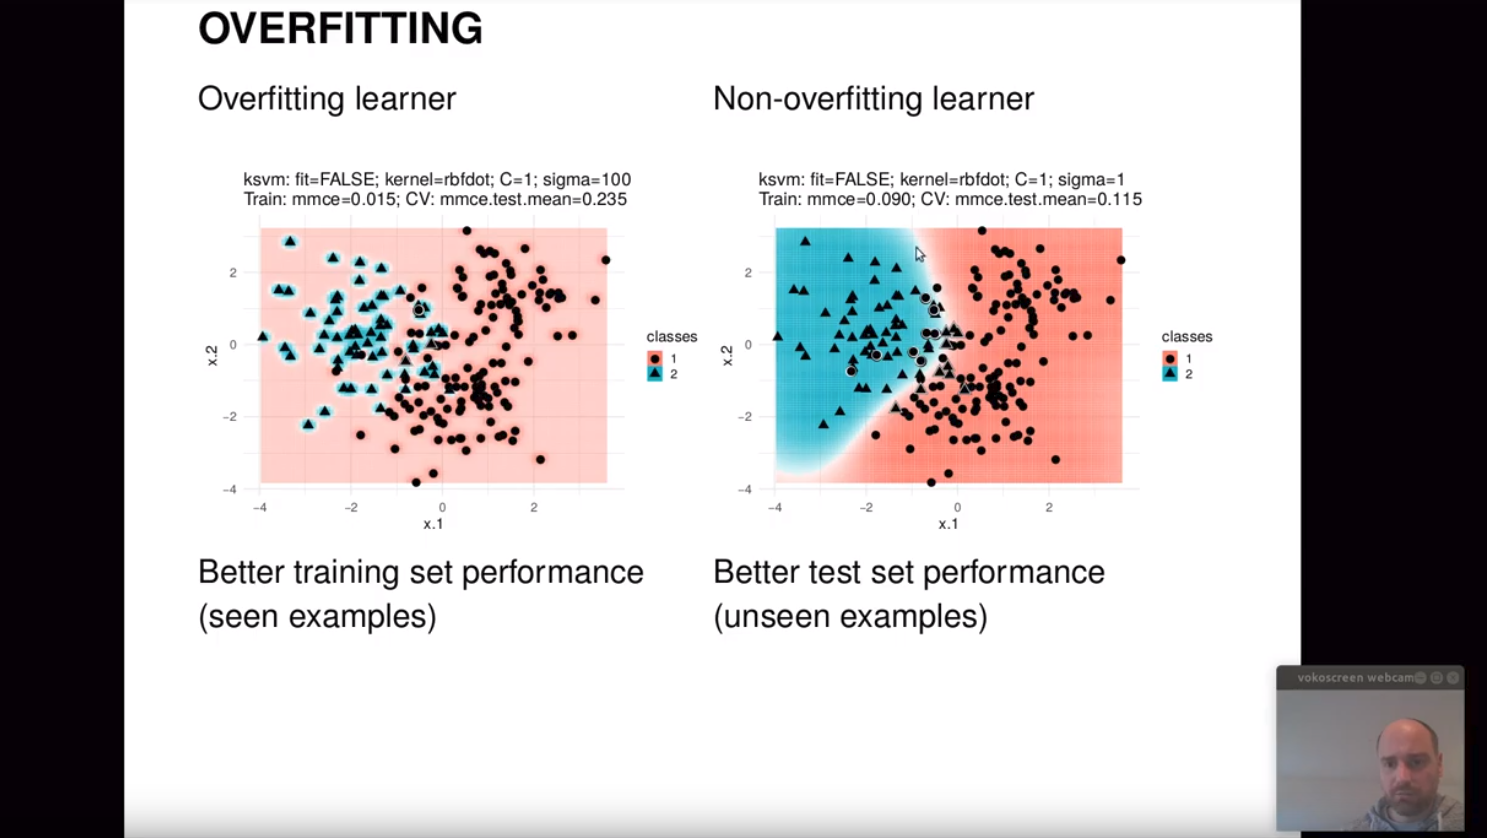
\includegraphics[width=\textwidth]{figures/iml_video.png}
  \end{center}

\end{frame}

\begin{frame}{Concept - Interactive Tutorials (Quiz)}

  \begin{center}
      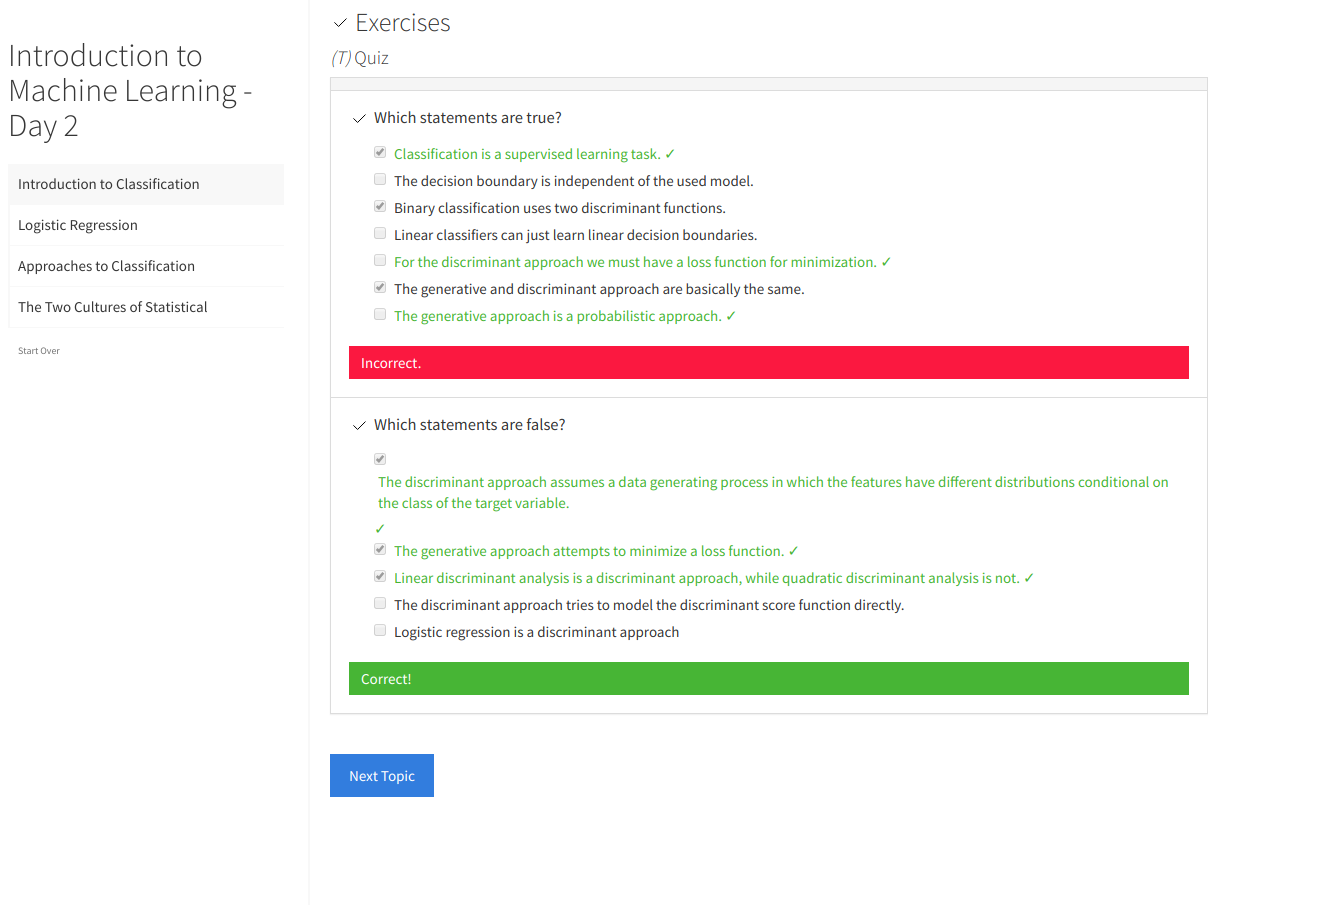
\includegraphics[width=\textwidth]{figures/iml_tut0.png}
  \end{center}

\end{frame}

\begin{frame}{Concept - Interactive Tutorials (Examples)}

  \begin{center}
      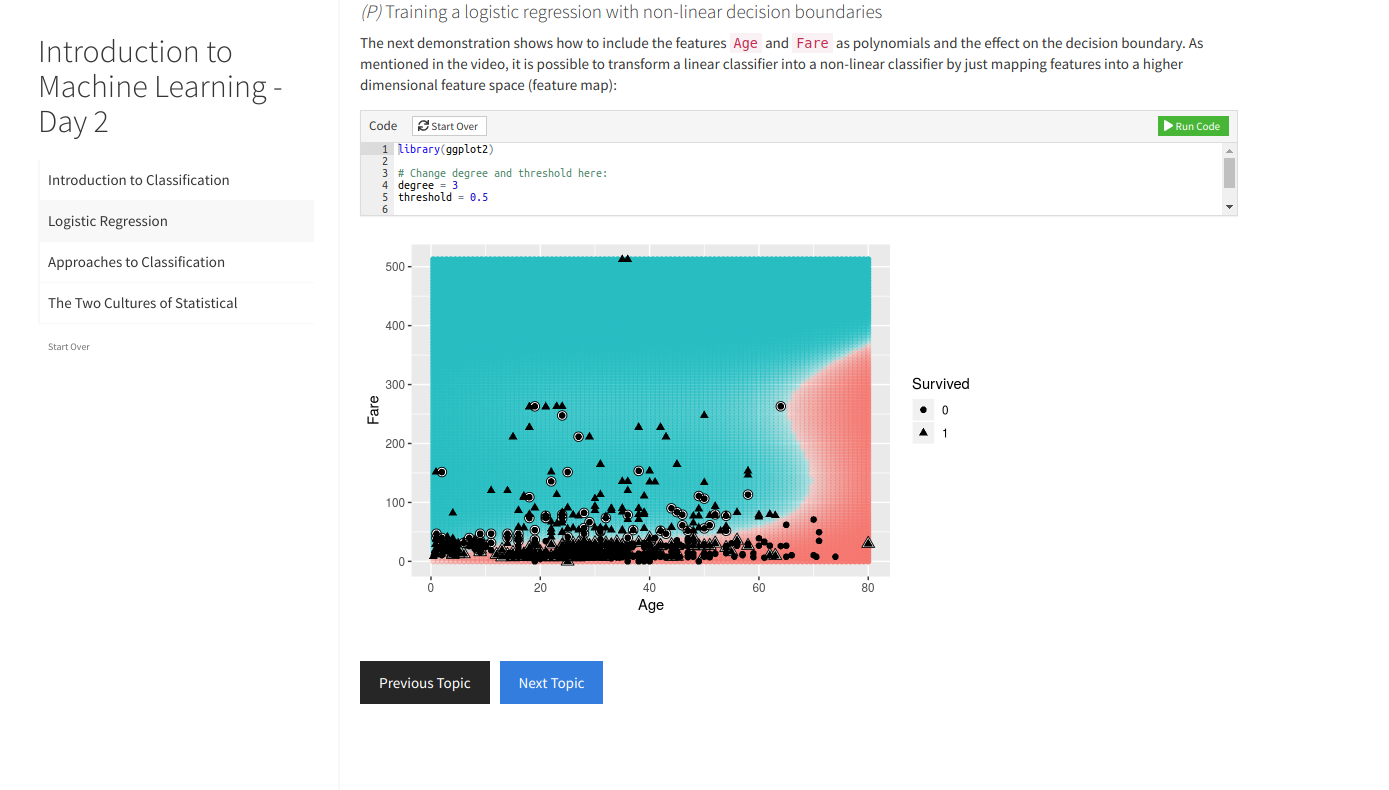
\includegraphics[width=\textwidth]{figures/iml_tut1.png}
  \end{center}

\end{frame}

\begin{frame}{Outlook}
  \begin{itemize}
      \item Cut lectures / videos down to smaller chunks
      \item Collaborative development with other lecturers / sites
      \item More code demos
      \item Better auto-correction of programming exercises
      \item Advertise material to other LMU departments / programs
  \end{itemize}

\end{frame}

\end{document}
